\documentclass[20pt]{report}
%\usepackage[paperwidth=37cm,paperheight=37cm]{geometry}
%\usepackage[a4paper,vmargin={20mm,20mm},hmargin={20mm,10mm}]{geometry}
\usepackage{geometry}
\usepackage{hyperref}
 \geometry{
 a4paper,
 total={210mm,297mm},
 left=20mm,
 right=20mm,
 top=20mm,
 bottom=20mm,
 }
\usepackage{graphicx}
\usepackage{hyperref}
\hypersetup{
    colorlinks=true,
    linkcolor=black,
    citecolor=black,
    filecolor=black,
    urlcolor=blue,
}

%\graphicspath{{C:/Users/Akhil Jain/Desktop/Pics/}}
\begin{document}

\title{\textbf{\LARGE{Programming Firebird-V from Linux Platform} \vspace{0.3in} \\  E-Yantra Summer Internship  Program}}
\author{Team:\hspace{0.1in} Akhil Jain \hspace{0.2in} Anshul Panjabi \\ \vspace{0.2in}  Mentors: \vspace{0.05in} Saurav S. \hspace{0.2in} Thyagarajan R.}

\date{\today}

\maketitle

\newpage
\chapter{Firebird V ARM Linux Programming}
\section{Generation of bin files for ARM in Linux}
\begin{enumerate}
\item Install GNU-arm toolchain by typing the following commands on the terminal:
\newline
\textbf{sudo add-apt-repository ppa:terry.guo/gcc-arm-embedded\\sudo apt-get update\\sudo apt-get install gcc-arm-none-eabi}
\item Install and configure Eclipse and install the GNU-ARM-Eclipse plugins as shown on this webpage:
\newline
\url{http://gnuarmeclipse.livius.net/blog/plugins-install/}
\item Open file menu and select New > C Project. You will see a window shown in fig. \ref{ecl1}.
\begin{figure}[!h]
\centering
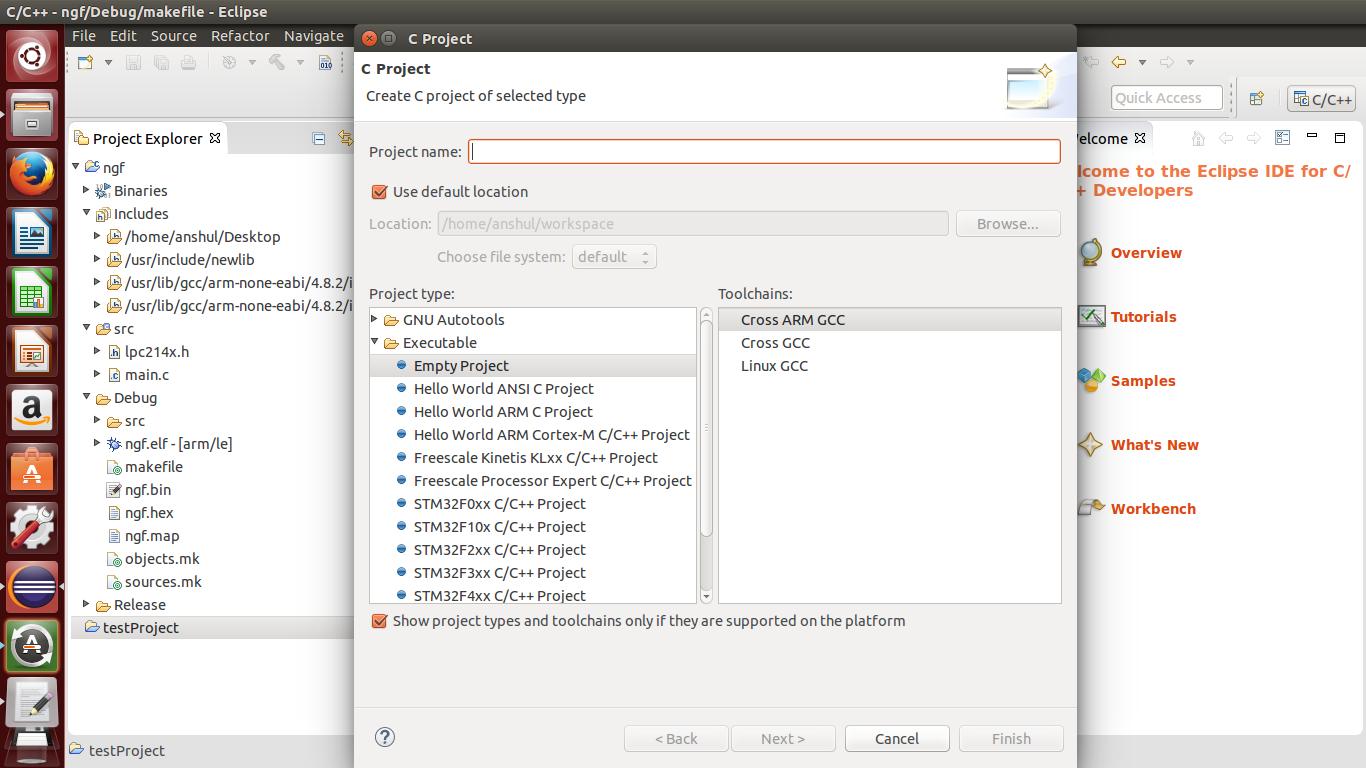
\includegraphics[width=0.7\linewidth]{ecl1}
\caption{C Project}
\label{ecl1}
\end{figure}
\item Give a project name and author name as shown in fig. \ref{ecl2}.
\begin{figure}[!h]
\centering
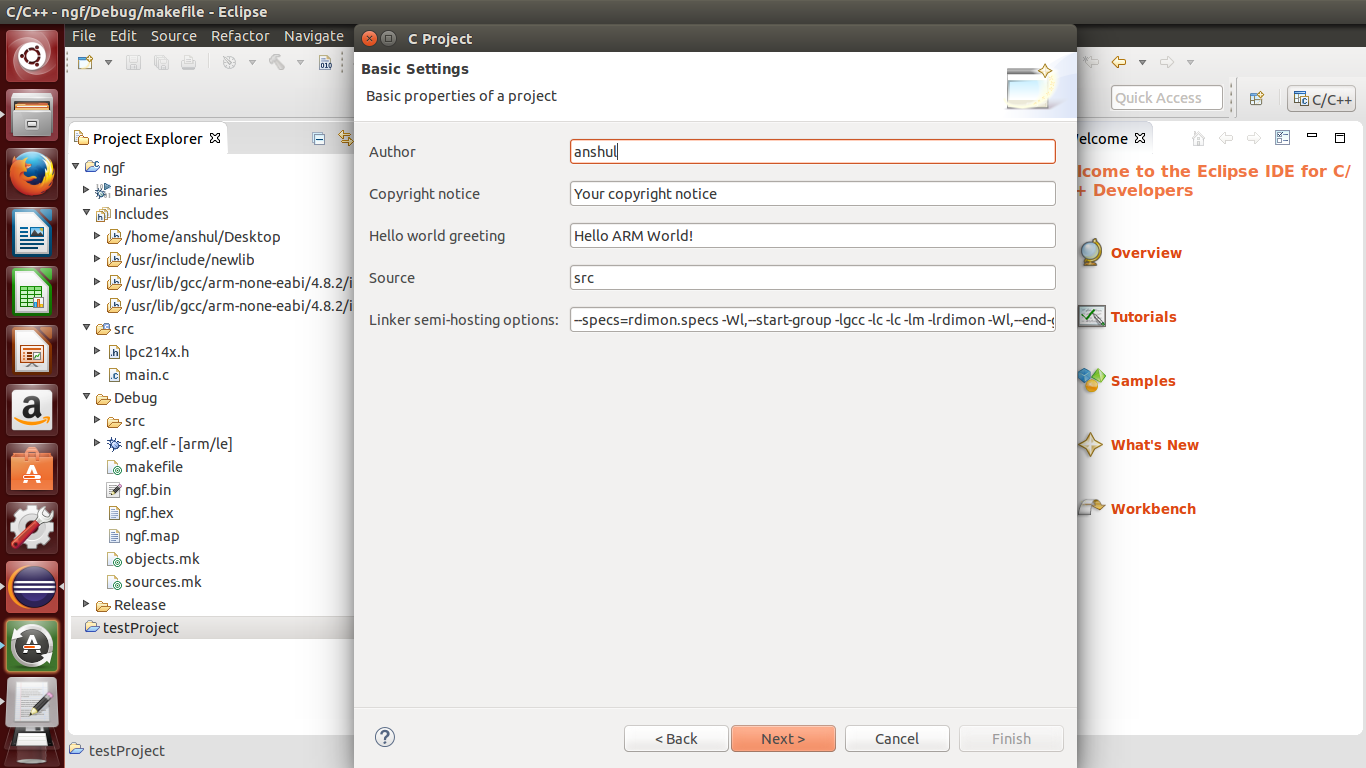
\includegraphics[width=0.7\linewidth]{ecl2}
\caption{Basic Settings}
\label{ecl2}
\end{figure}
\item Click Next to continue as shown in fig \ref{ecl3}. 
\begin{figure}[!h]
\centering
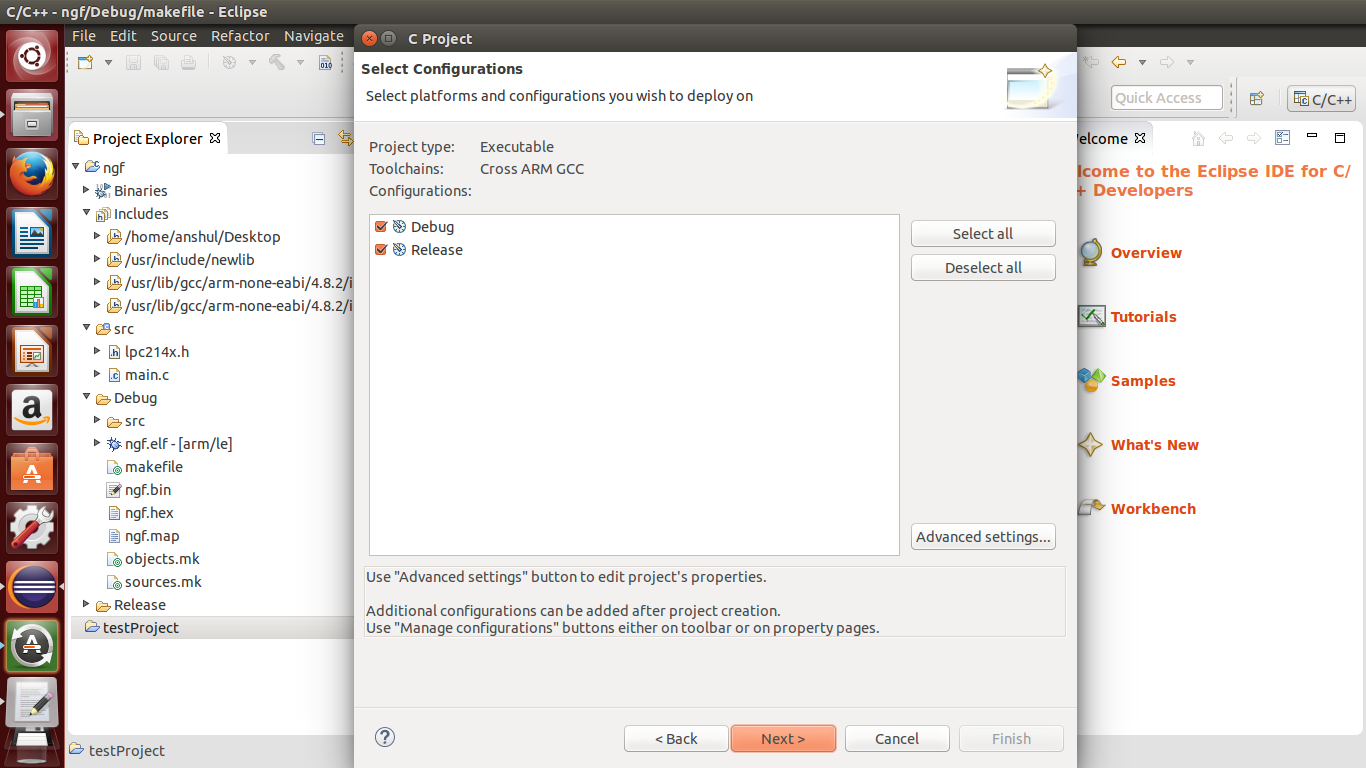
\includegraphics[width=0.7\linewidth]{ecl3}
\caption{Select Configurations}
\label{ecl3}
\end{figure}

\item Select options as shown in fig. \ref{ecl4} and click on Finish.
\begin{figure}[!h]
\centering
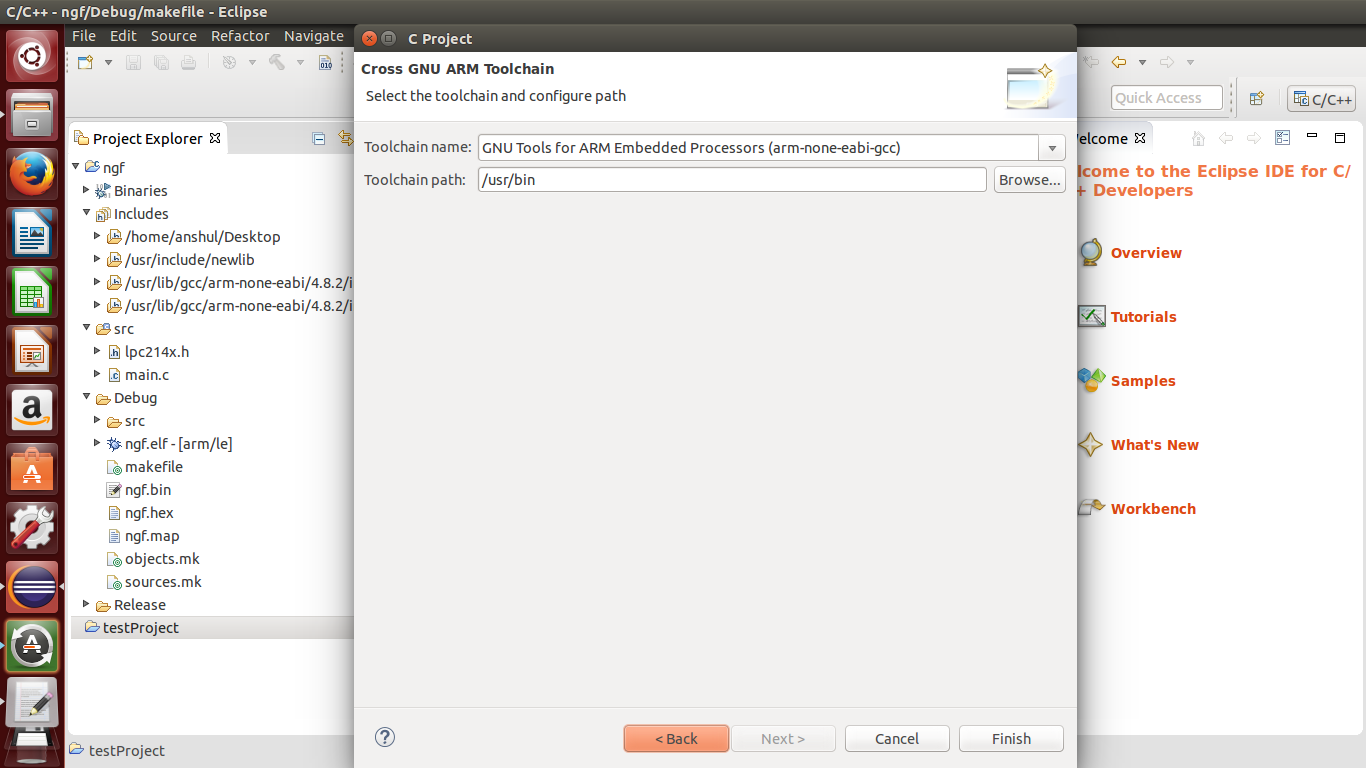
\includegraphics[width=0.7\linewidth]{ecl4}
\caption{Cross GNU ARM Toolchain}
\label{ecl4}
\end{figure}
\item Right Click on the project folder in the project explorer window of Eclipse and select properties.
\item Configure the target processor as shown in fig. \ref{ecl5}.
\begin{figure}[!h]
\centering
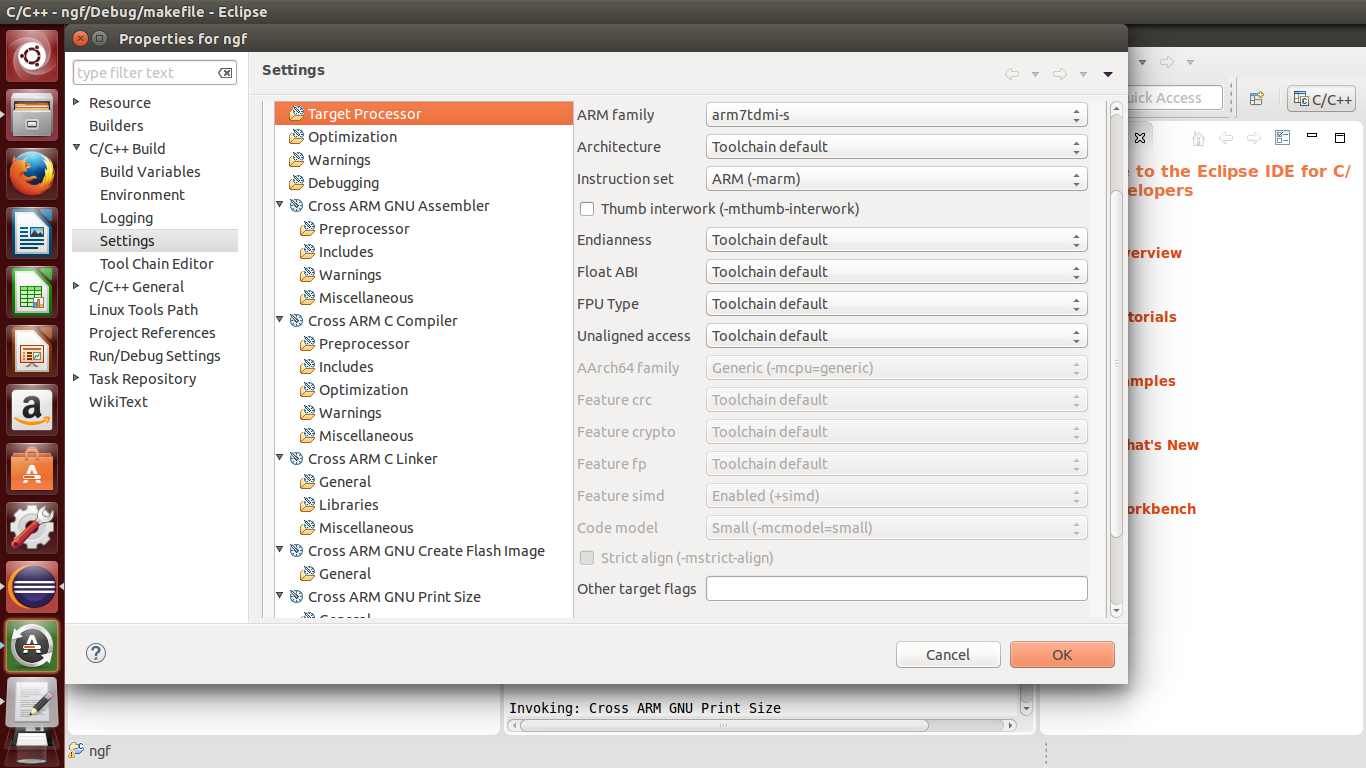
\includegraphics[width=0.7\linewidth]{ecl5}
\caption{Configuring Target Processor}
\label{ecl5}
\end{figure}
\item Configure the output file format as shown in fig. \ref{ecl6}.
\begin{figure}[!h]
\centering
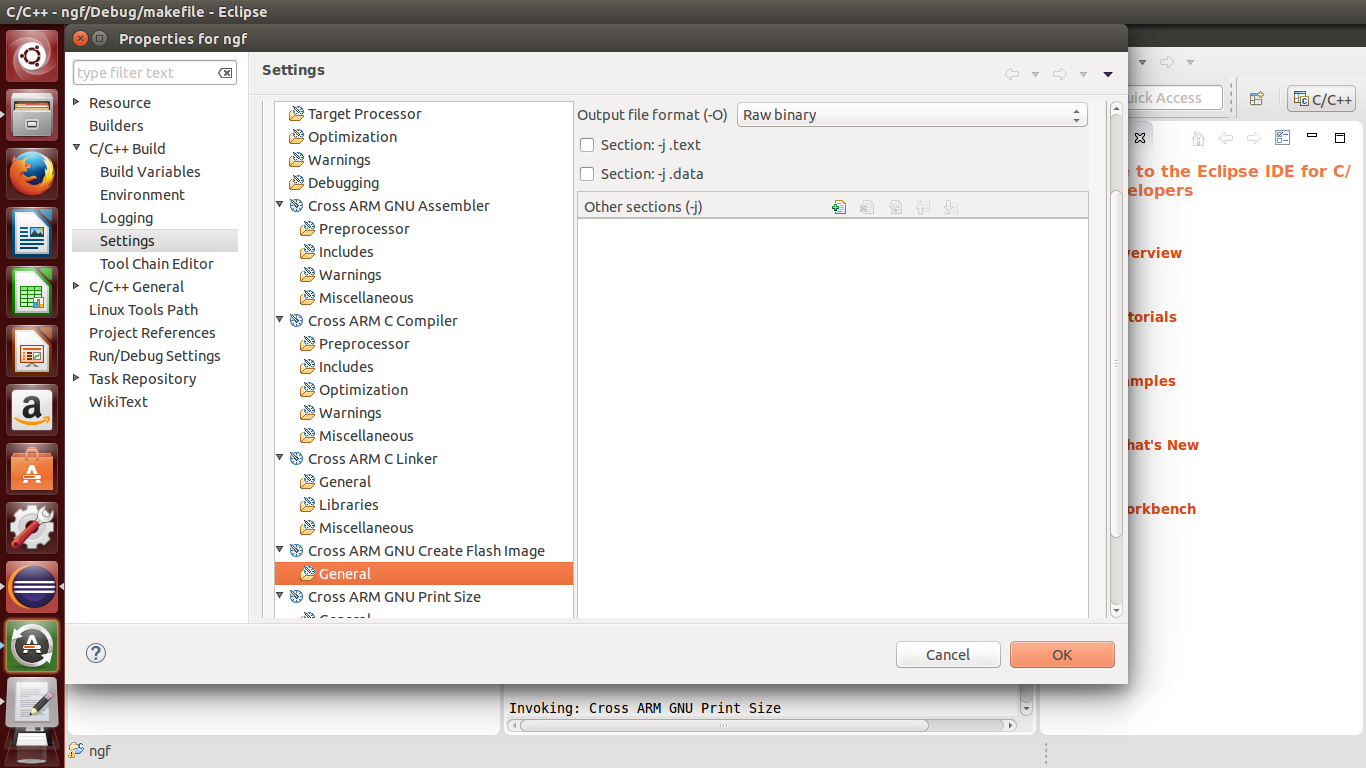
\includegraphics[width=0.7\linewidth]{ecl6}
\caption{Configuring Output file format}
\label{ecl6}
\end{figure}
\item Add the linker script file as shown in fig. \ref{ecl7}.
\begin{figure}[!h]
\centering
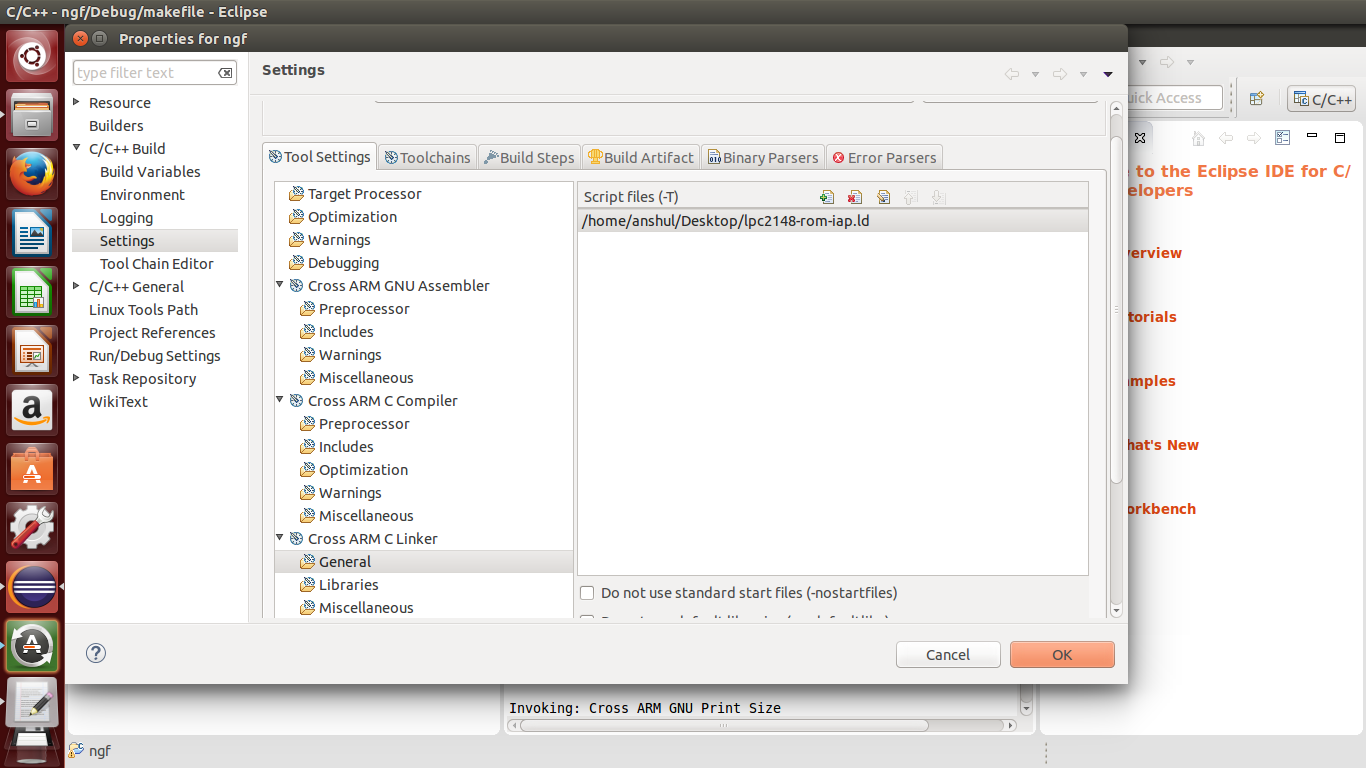
\includegraphics[width=0.7\linewidth]{ecl7}
\caption{Adding a Linker Script file}
\label{ecl7}
\end{figure}
\item Add the path to the 'lpc214x.h' header file as shown in fig. \ref{ecl8}.
\begin{figure}[!h]
\centering
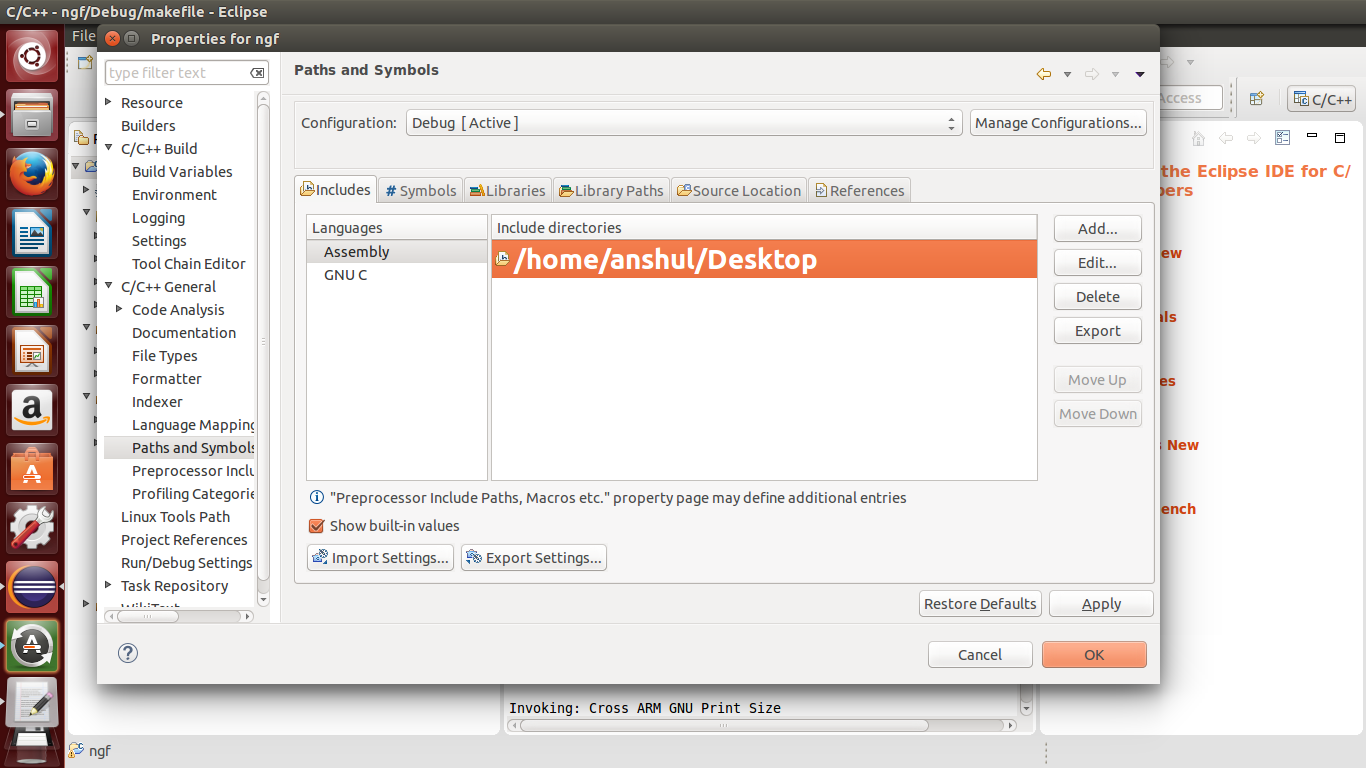
\includegraphics[width=0.7\linewidth]{ecl8}
\caption{Adding the path to the lpc214x.h header file}
\label{ecl8}
\end{figure}
\item Write the program in main.c.
\item You can then click on the hammer icon as shown in fig. \ref{ecl9} to build your program.
\begin{figure}[!h]
\centering
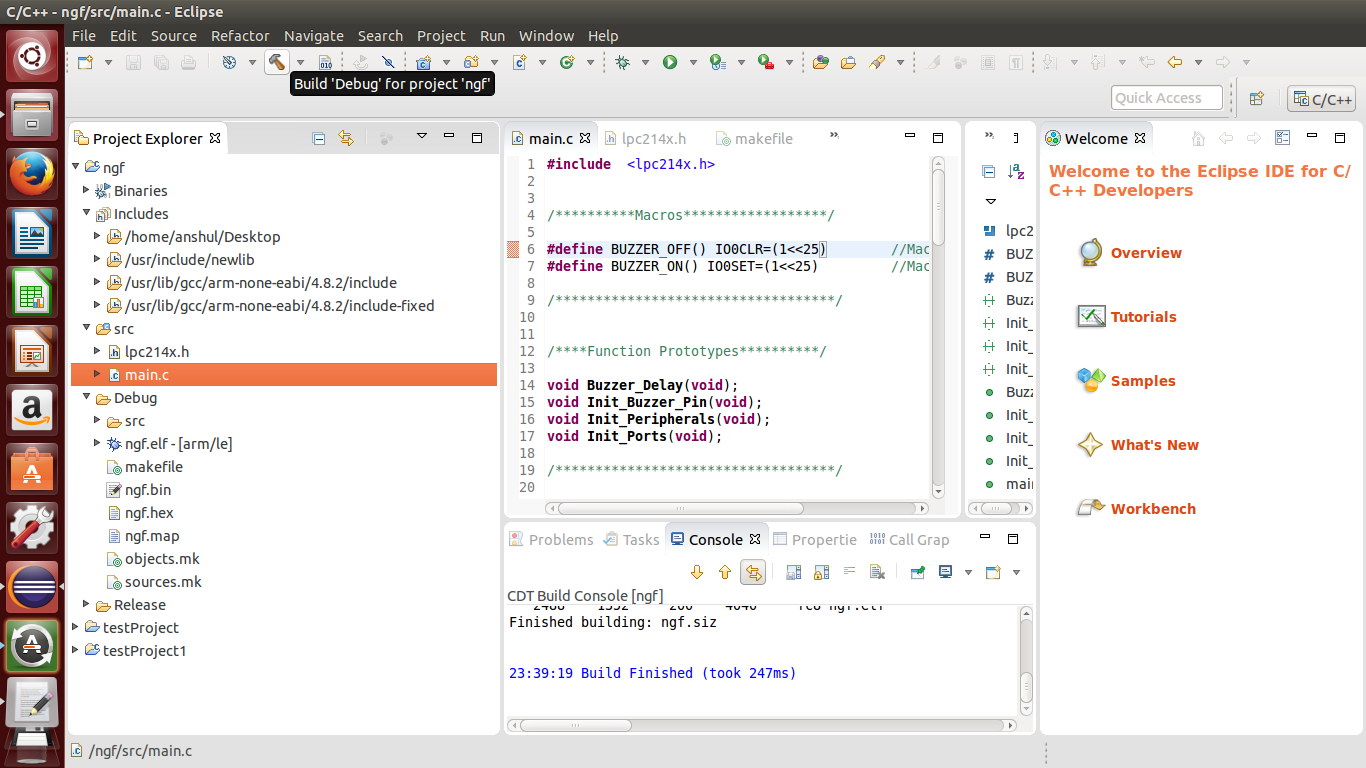
\includegraphics[width=0.7\linewidth]{ecl9}
\caption{Building the project}
\label{ecl9}
\end{figure}
\end{enumerate}

\textbf{Bugs:}
\begin{itemize}
\item Project cannot be built with the linker script, and without linker script it builds fine, but when loaded on the microcontroller, it won't work.
\end{itemize}


\section{\textbf{Loading generated bin file for ARM with Linux}}
\medskip

\begin{itemize}
\item Connect the LPC2148 firebird robot to USB port and enter the boot sequence for using IAP mode.
\item Open a terminal window, and navigate to the directory containing the bin file using cd command and then enter the following command(Here the LPC2148 Firebird V was mounted at /media/CRP DISABLD and contained a firmware.bin file):
\end{itemize}

\medskip

\textbf{dd conv=nocreat,notrunc if=newfile.bin of=/media/CRP\ DISABLD/firmware.bin}

\medskip
\medskip

\textbf{References:}
\begin{itemize}
\item \url{http://gnuarmeclipse.livius.net/blog/}
\item \url{http://sourceware-org.1504.n7.nabble.com/Problem-linking-with-static-libraries-for-arm-elf-td152499.html}
\item \url{https://groups.google.com/forum/#!topic/fabathome-forums/gwEFoVKh-hw}
\item \url{https://github.com/jeffreyantony/pymite-lpc2148/blob/master/Makefile}
\item \url{http://openlpc.com/4e26f1/reference}
\end{itemize}
\end{document}